\section{Expected Limits}

We have used the methodology described in this note and in a prior analysis~\cite{CMS_AN_2009-070} to 
determine our expected limits with more integrated luminosity.  For the expected limits the PYTHIA MC
samples discussed previously were used for the background, but otherwise the analysis is the same 
as just described.  We form smooth samples background samples without fluctuations from a smooth fit
to the QCD data and use the number of events expected in each bin from this smooth fit to perform
the analysis.  The expected upper limits on the cross section are shown in Fig.~\ref{future_limit}
compared to 7 models of resonance.   The mass limit expected for each model occurs where the expected
upper limit on the cross section for the appropriate parton pair crosses the model cross section curve.
These expected 95\% CL mass limits are plotted in Figure~\ref{future_mass_limit} as a function of integrated
luminosity. The slope and functional form of the mass limit dependence
on integrated luminosity strongly depends on the parton distributions involved in the process. The $E_6$ diquark
process excluded mass limits curve vs. integrated luminosity is not linear like for $q^*$ and Colorons because
the $E_6$ diquark cross section slope vs. resonance mass changes appreciably in the region $0.5$ to $3$ TeV.
We have already surpassed the mass limit on string resonances set by the Tevatron, and 
with 400 nb$^{-1}$ we expect to reach the mass limit of 870 GeV for excited quarks also from the Tevatron.


%With 120 nb$^{-1}$ of data, our actual measured mass limit for string resonances, 
%$1.67$ TeV is in good agreement with the expected mass limits of $1.75$.  Our actual
%meaaured mass limit for excited quarks, $0.59$ TeV is slighly lower than the expected
%mass limit of $0.63$ TeV because of the single bin upward fluctuation in the data near
%$0.6$ TeV.  Converseley, our actual measured mass limit for axigluons and colorons, 
%$0.52$ TeV, is higher than our expected mass limit of $0.40$ TeV, because of 
%the downward fluctuation of the data around $0.5$ TeV.


\begin{figure}[!ht]
  \begin{center}
     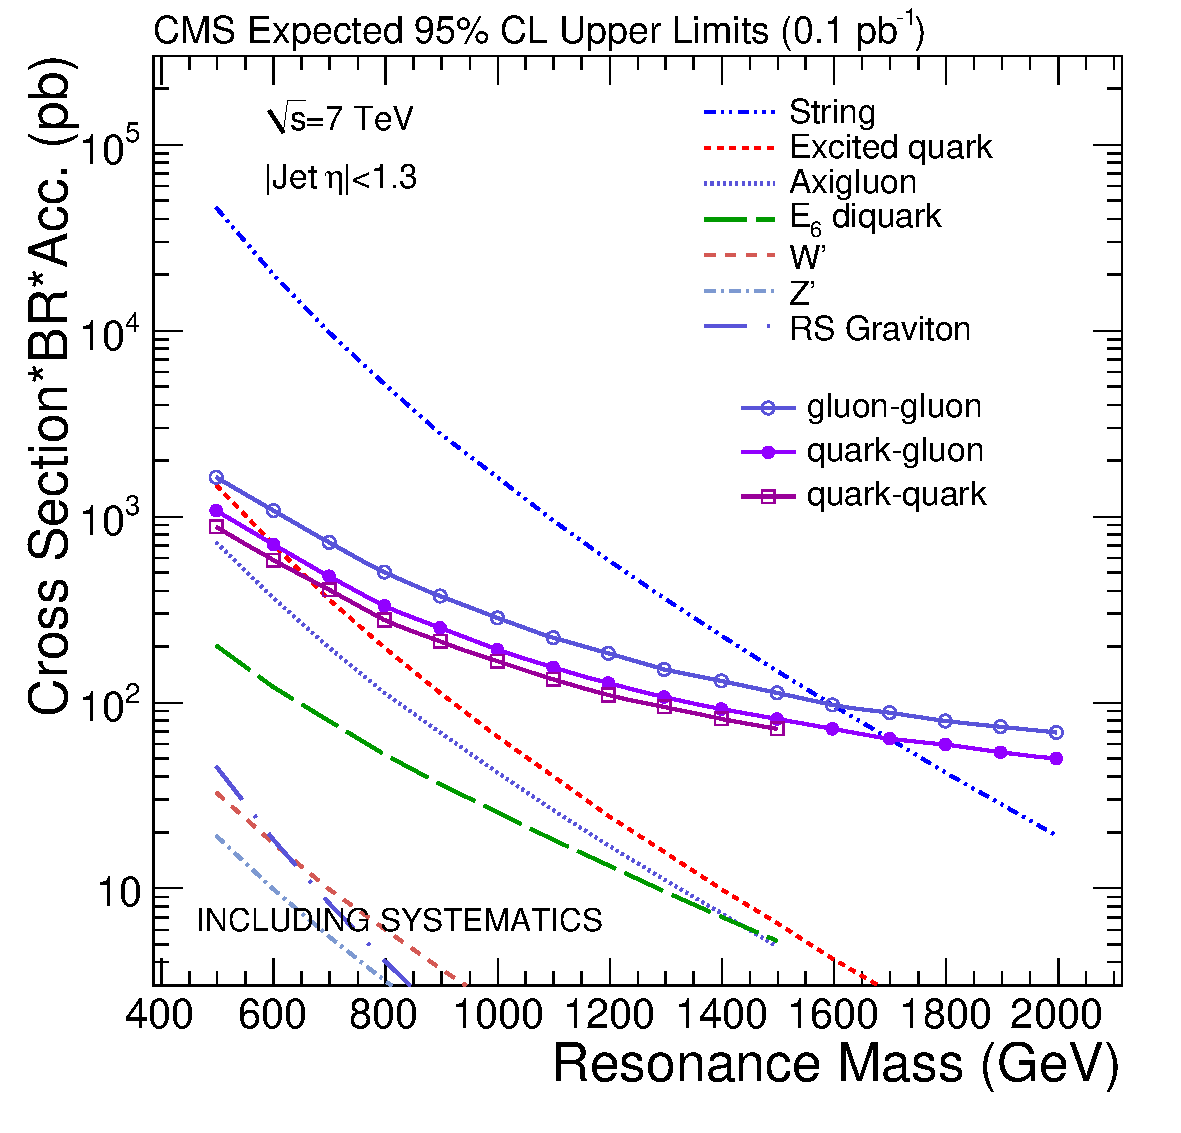
\includegraphics[width=0.48\textwidth]{Figures/Smooth_limit_including_sys_100nb.pdf}
     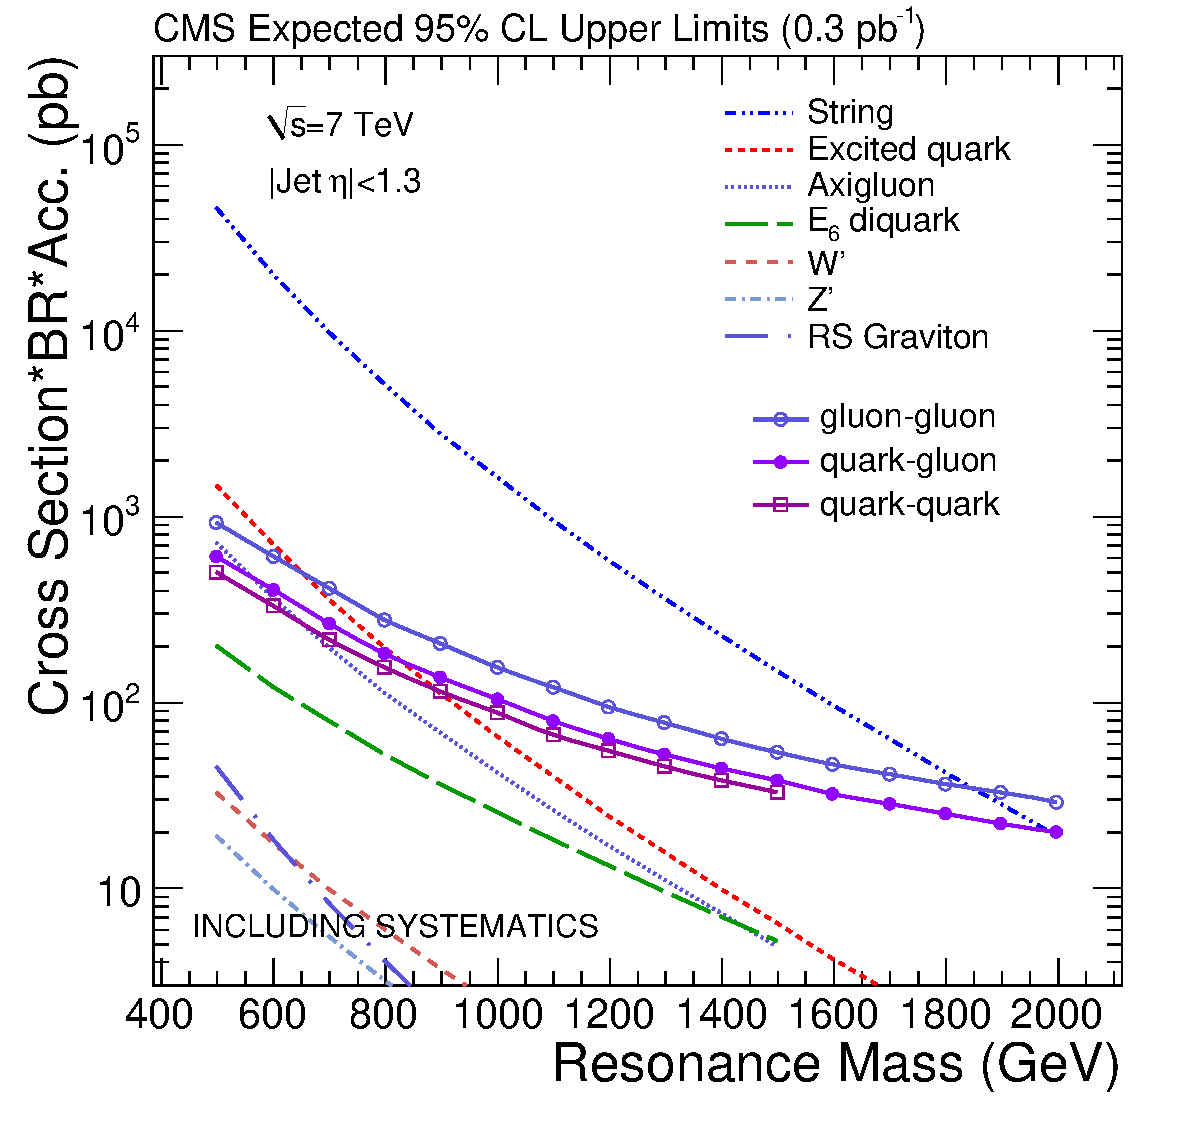
\includegraphics[width=0.48\textwidth]{Figures/Smooth_limit_including_sys_300nb.pdf}
     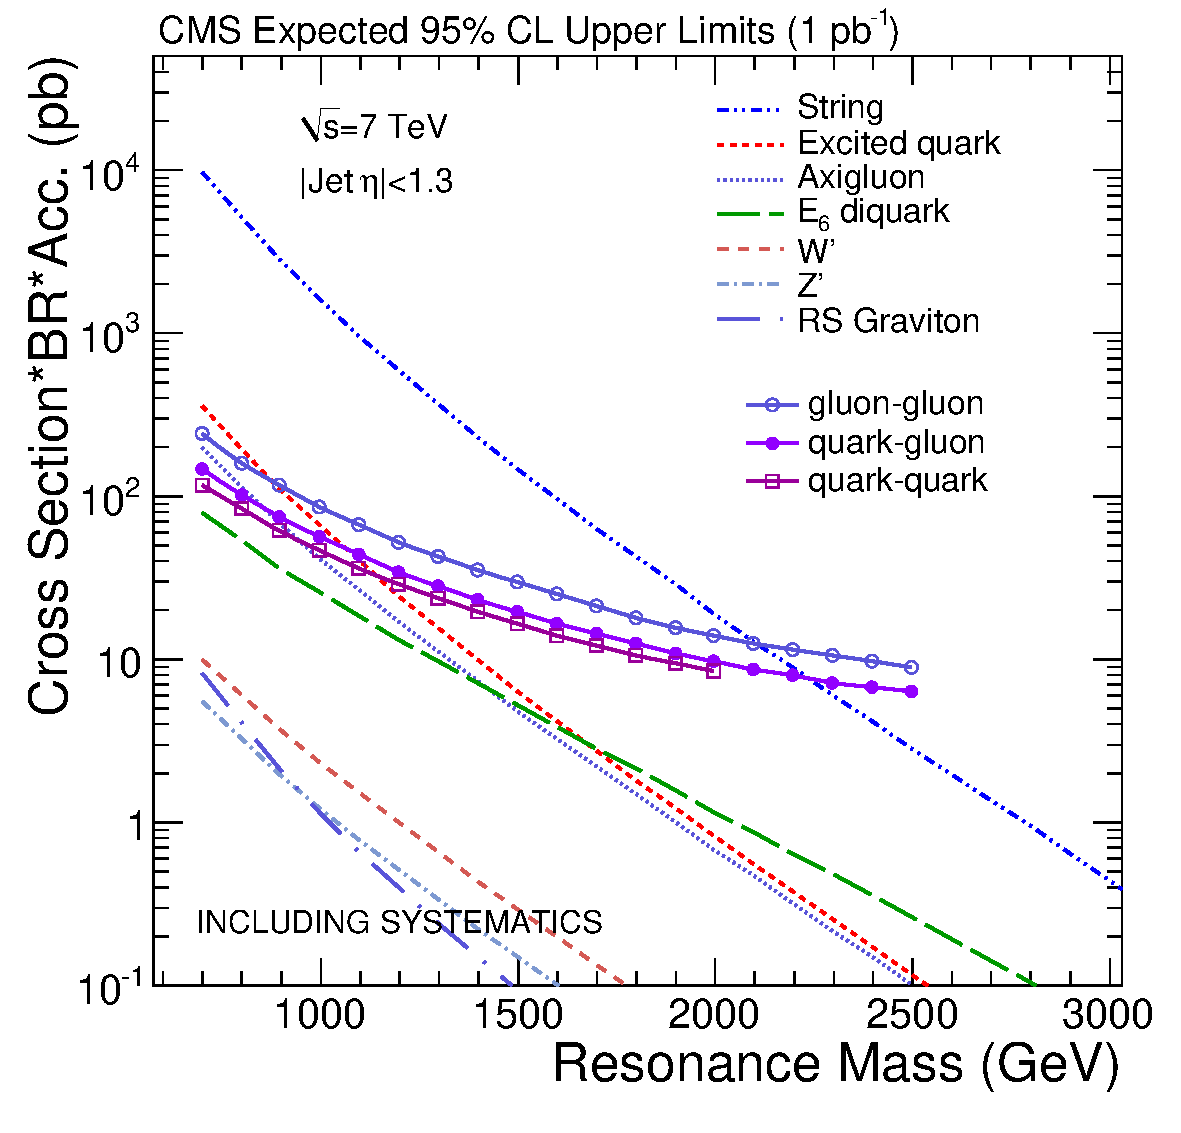
\includegraphics[width=0.48\textwidth]{Figures/Smooth_limit_including_sys_1pb.pdf}
     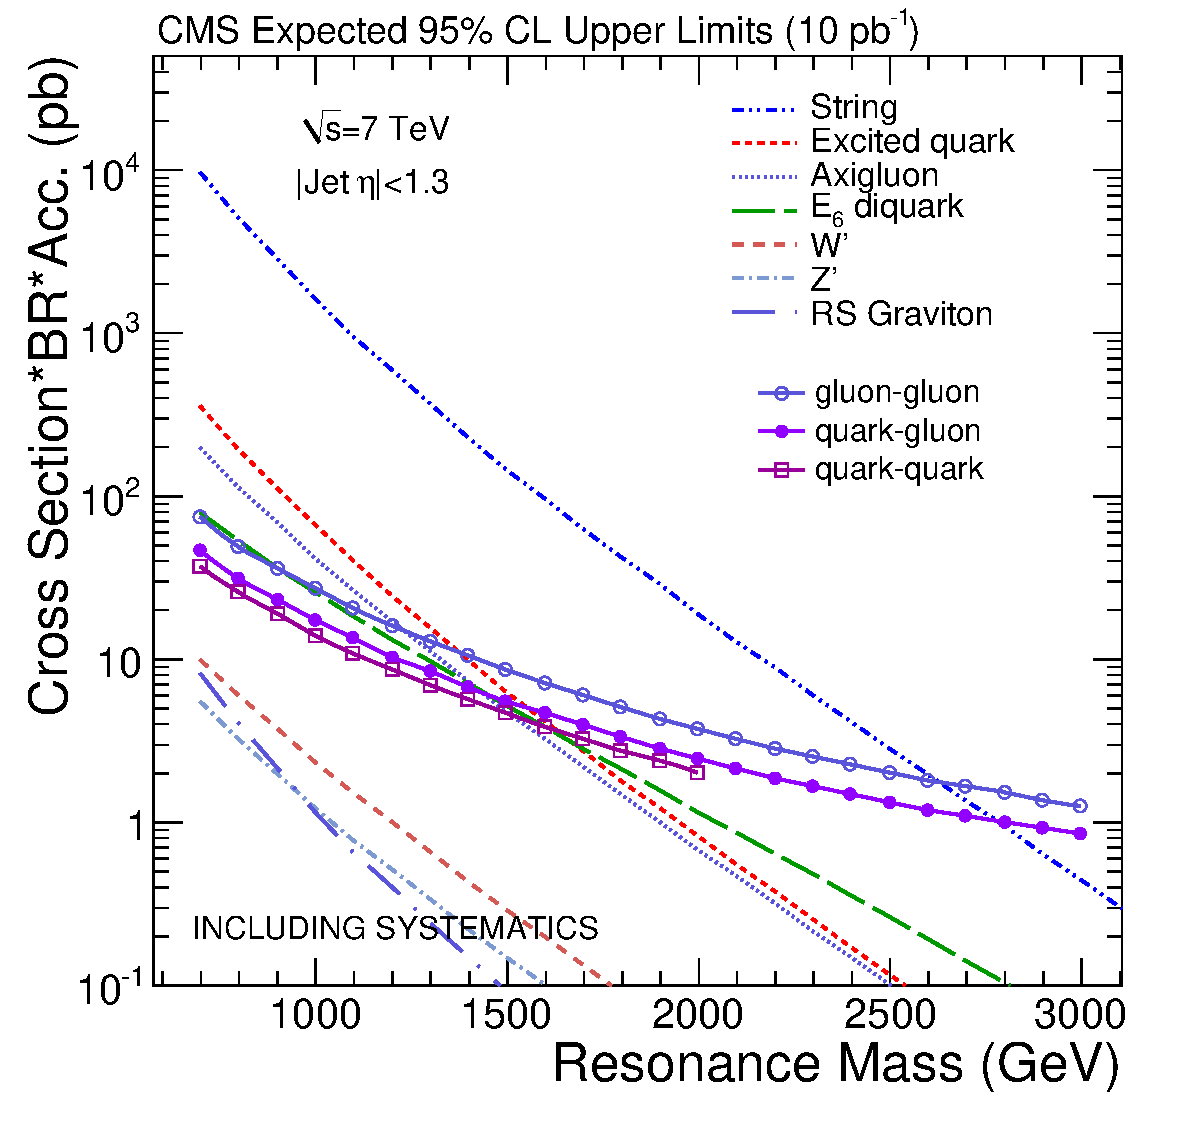
\includegraphics[width=0.48\textwidth]{Figures/Smooth_limit_including_sys_10pb.pdf}
     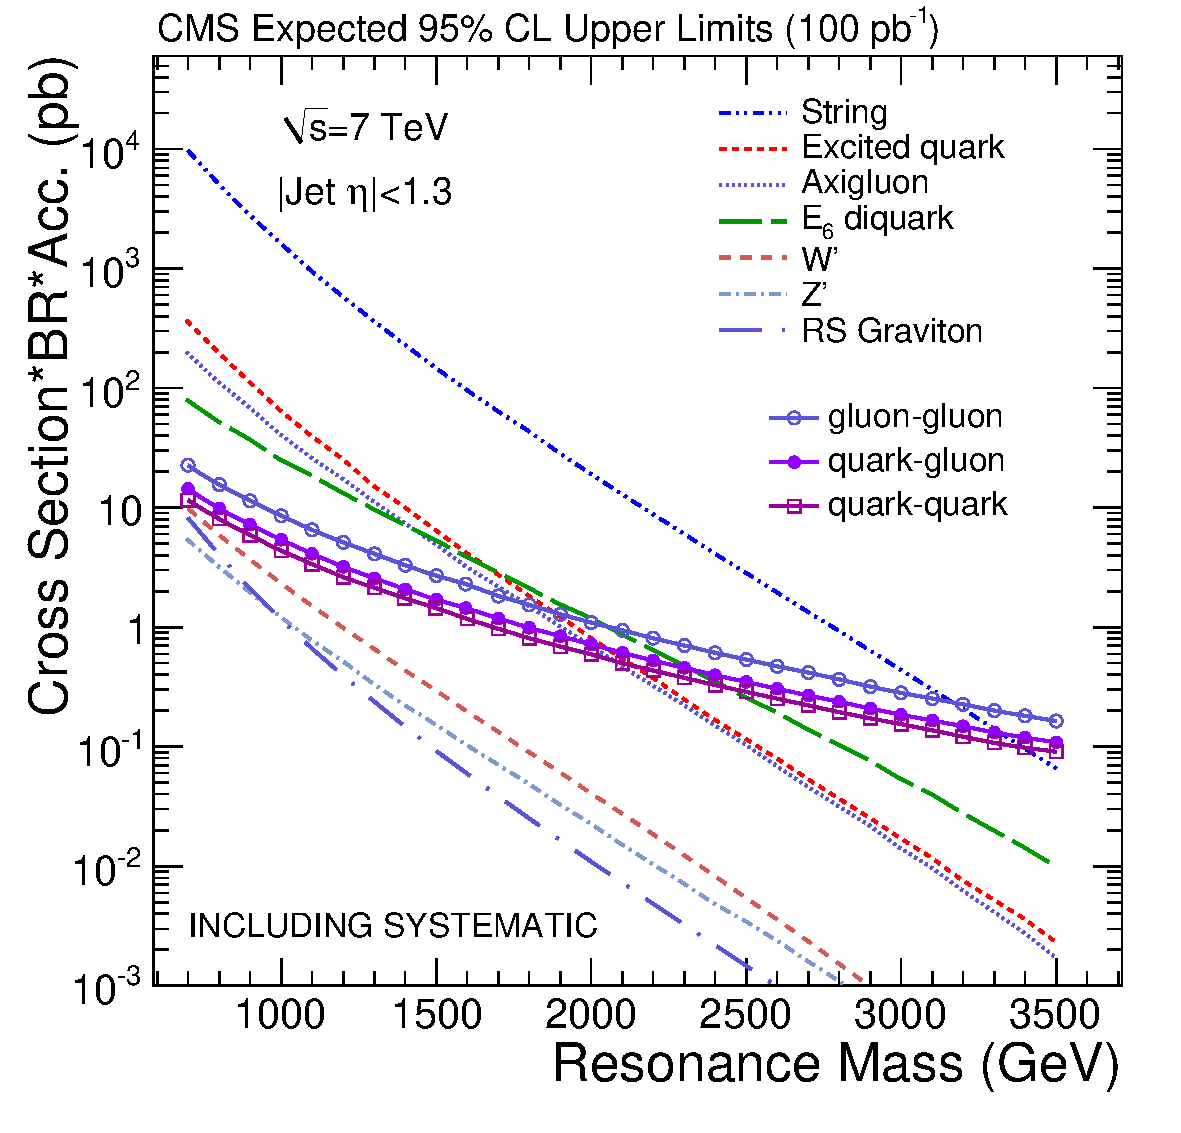
\includegraphics[width=0.48\textwidth]{Figures/Smooth_limit_including_sys_100pb.pdf}
     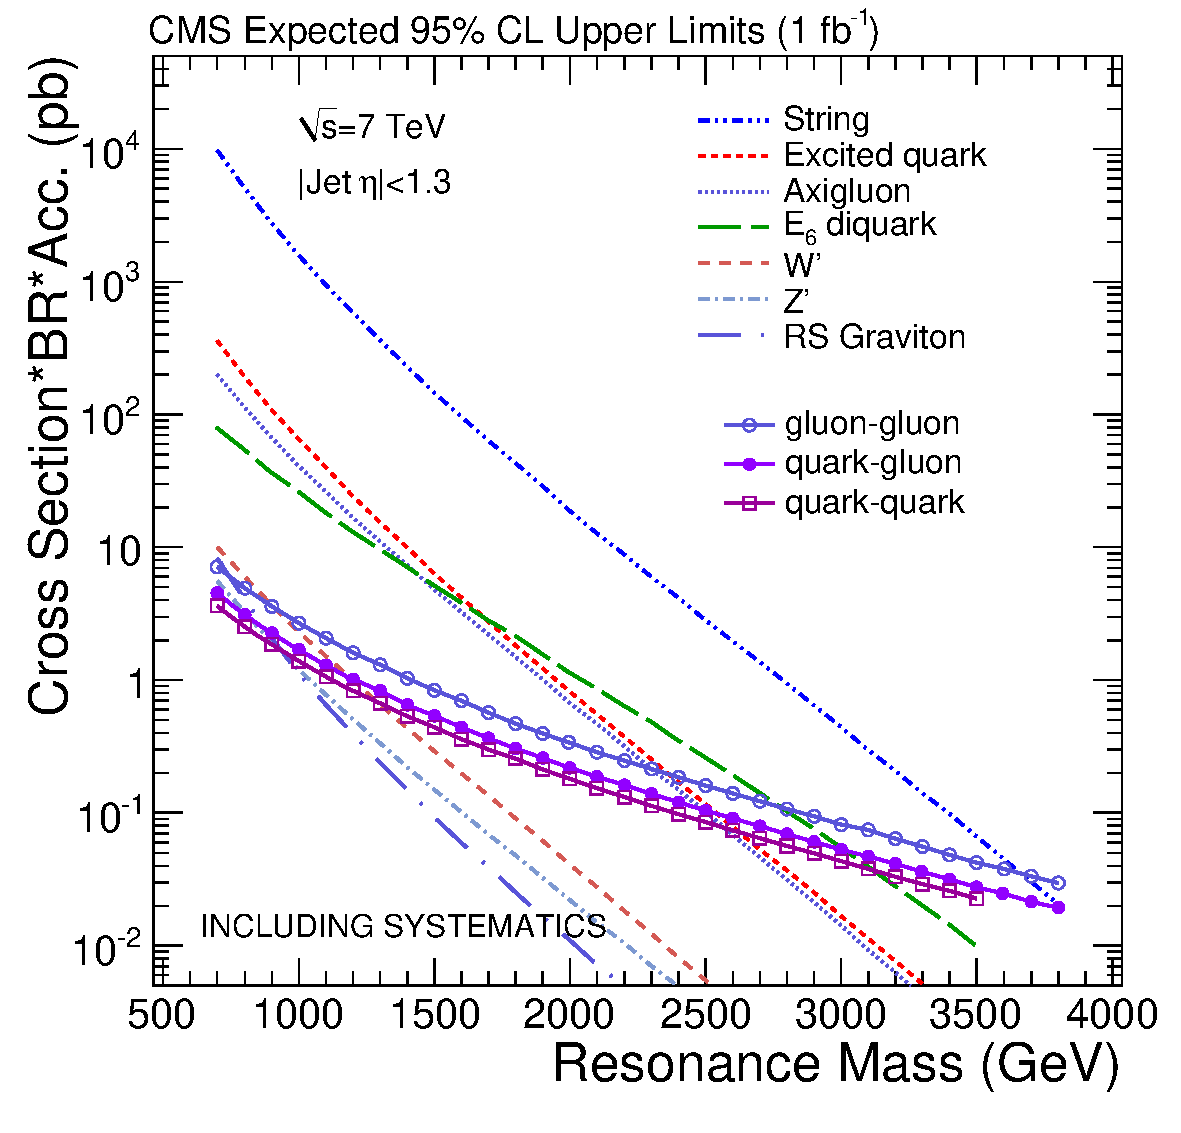
\includegraphics[width=0.48\textwidth]{Figures/Smooth_limit_including_sys_1fb.pdf}
    \caption{Model cross sections (curves) compared to the CMS expected upper 
    limits (points) at 6 different integrated luminosities:
    0.1,0.3, 1, 10, 100, and 1000 pb$^{-1}$.}
    \label{future_limit}
  \end{center}
\end{figure}

\begin{figure}[!ht]
  \begin{center}
     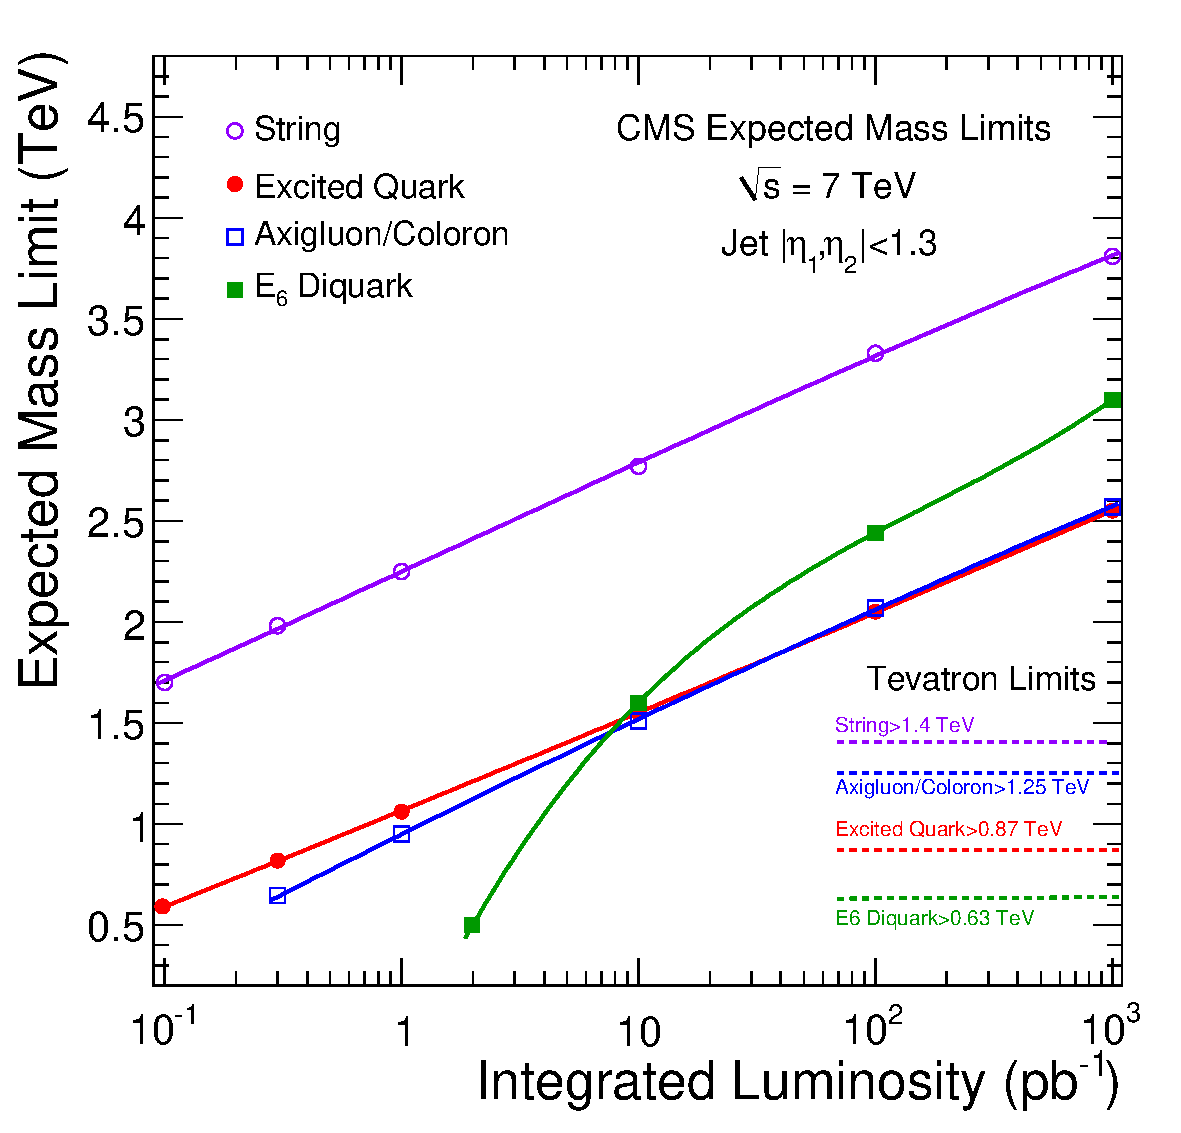
\includegraphics[width=\textwidth]{Figures/excluded_mass_limit.pdf}
    \caption{Expected excluded mass limits at 95\% CL vs. integrated luminosity for
    various various models.}
    \label{future_mass_limit}
  \end{center}
\end{figure}
